\subsection{Laplace Transformation}

\begin{mdframed}[style=exercise]
	\[
		x(t) \laplace \underline{X}(s)
	\]
	Hintransformation - Analysegleichung
	\[
		\underline{X}(s) = \mathcal{L}\left\{ x(t) \right\} = \int_0^\infty x(t) e^{-st} dt
	\]
	Rücktransformation - Synthesegleichung:
	\[
		x(t) = \mathcal{L}^{-1}\left\{ \underline{X}(s) \right\} = \frac{1}{2\pi j}\int_{\sigma-j\infty}^{\sigma+j\infty} \underline{X}(s) e^{-st} ds
	\]
\end{mdframed}

\subsubsection{Eigenschaften Laplace Transformation}
\begin{mdframed}[style=exercise,nobreak=false]
	\begin{itemize}
		\item \textbf{Linearität}
		      \[
			      \alpha x_1(t) + \beta x_2(t) \ \laplace\  \alpha \underline{X}_1(t) + \beta \underline{X}_2(t)
		      \]
		      \vspace{-1.5em}
		\item \textbf{Skalierung im Zeitbereich}
		      \[
			      x(\alpha t) \ \laplace\  \frac{1}{\alpha} \underline{X}\left(\frac{s}{\alpha}\right) \qquad \color{red}{\alpha > 0}
		      \]
		      \vspace{-1.5em}
		\item \textbf{Skalierung im Bildbereich}
		      \[
			      \frac{1}{\alpha}x\left(\frac{t}{\alpha}\right)\ \laplace\ \underline{X}(\alpha s) \qquad \color{red}{\alpha > 0}
		      \]
		      \vspace{-1.5em}
		\item \textbf{Verschiebung im Zeitbereich}
		      \[
			      x(t-t_0)\ \laplace\ e^{-st_0} \underline{X}(s) \qquad \color{red}{t_0 > 0}
		      \]
		      \vspace{-1.5em}
		\item \textbf{Verschiebung im Bildbereich - Modulation}
		      \[
			      e^{at}x(t) \ \laplace\ \underline{X}(s-a)
		      \]
		      \vspace{-1.5em}
		\item \textbf{Faltung}
		      \[
			      x_1(t)*x_2(t) \ \laplace\ \underline{X}_1(s)\cdot \underline{X}_2(s)
		      \]
		      \vspace{-1.5em}
		\item \textbf{Differentiation im Zeitbereich}
		      \[
			      \frac{d}{dt}x(t) \ \laplace\ s\cdot\underline{X}(s)\color{red}{-x(0^+)}
		      \]
		      \vspace{-1.5em}
		\item \textbf{Differentiation im Bildbereich}
		      \[
			      t\cdot x(t) \ \laplace\ -\frac{d}{ds}\underline{X}(s)
		      \]
		      \vspace{-1.5em}
		\item \textbf{Integration im Zeitbereich}
		      \[
			      \int_0^t x(\tau)d\tau \ \laplace\ \frac{1}{s}\underline{X}(s)
		      \]
		      \vspace{-1.5em}
		\item \textbf{Integration im Bildbereich}
		      \[
			      \frac{1}{t}x(t) \ \laplace\ \int_s^\infty\underline{X}(s)ds
		      \]
	\end{itemize}
\end{mdframed}
\subsubsection{Rücktransformation rationaler Funktionen}
\footnotesize
Partialbruchzerlegung: Siehe papula nach S.157

\normalsize
\subsection{LTI-Systeme im Bildbereich}
\begin{center}
    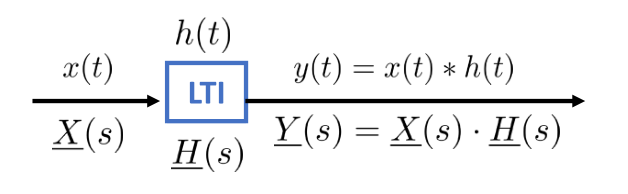
\includegraphics[width=0.6\columnwidth]{Bilder/LTI_Systeme_im_Bildbereich.png}
\end{center}

\subsubsection{Impuls- und Sprungantwort im Bildbereich}
Impulsantwort:
\[
    h(t)\ \laplace\ \underline{H}(s)
\]
durch integrationssatz:
\[
    g(t) = \int_0^t h(\tau) d\tau
\]
Sprungantwort:
\[
    g(t)\ \laplace\ \frac{\underline{H}(s)}{s}
\]


\subsection{Systemantwort von LTI Systemen}
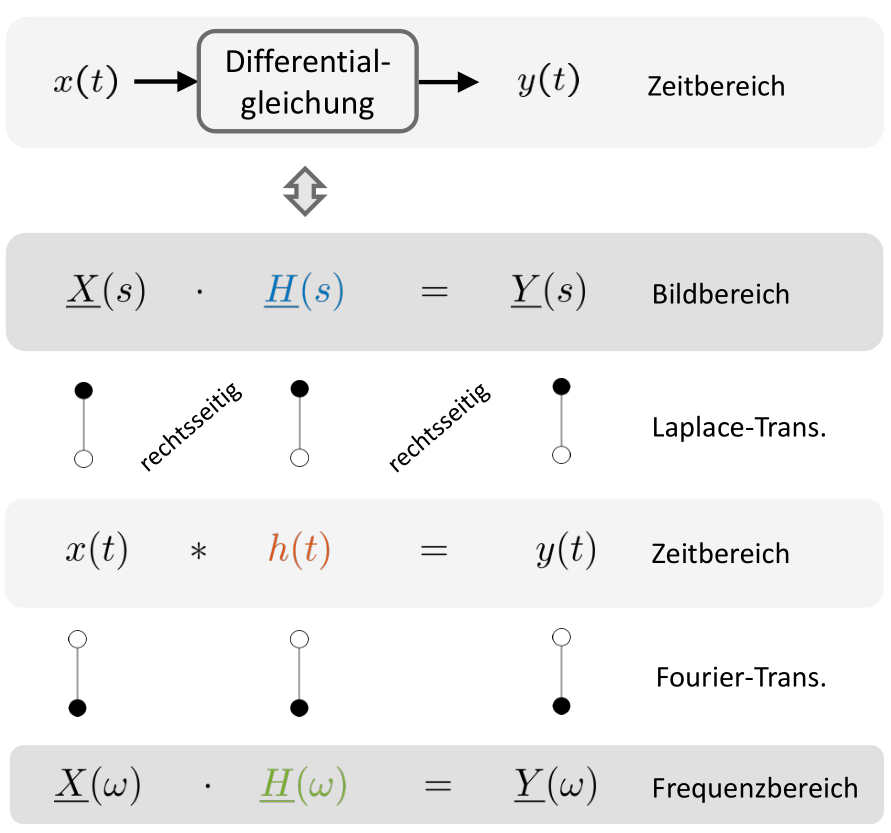
\includegraphics[width=0.98\columnwidth]{Bilder/LTI_Systemantworten.png}
